\section{Software Architecture}
 \label{section:sw-arc}

As the requirement is clear and the components of the system are defined, a software architecture is needed. A software architecture plays a major role in a software development project by providing a structure on how the software should be built and decisions made during this stage would be vital for the development process going forward. As Garlan wrote in one of his work \emph{Software Architecture}, a software architecture \enquote{plays a key role as a bridge between requirements and implementation.}\autocite{garlan-2000} A software architecture diagram is therefore created to help visualize the structure, functions and role of each component of the system.

\begin{figure}[h]
 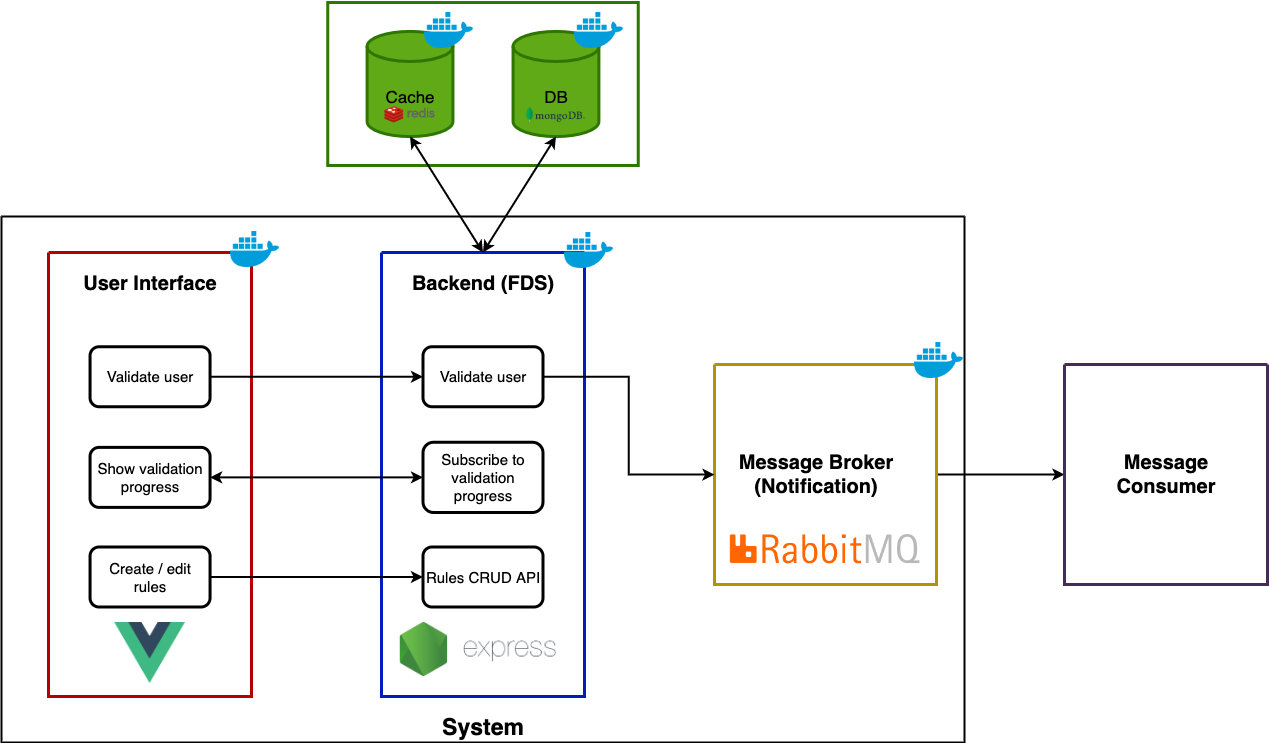
\includegraphics[width=\textwidth]{diagrams/sw-arc.png}
 \caption{Software architecture diagram}
 \label{fig:sw-arc}
\end{figure}

In a real world production environment, the user interface might need to be separated into several independent applications. A dedicated app to manage validation rules should be reachable only for internal employees (such as a developer from the company) while a customer facing UI that contains a registration form could also trigger a validation process directly after a new registration. An additional UI to display the progress of the currently running validation processes could also be built specifically for security agents of the companys, so that a fast reaction on certain suspicious customers can be done. For this project, all the use cases mentioned above will be implemented and combined into a single web application. 

The fraud detection service (\emph{backend, FDS}) is the core engine of the system where validation processes would be run. The FDS is responsible for all CRUD operations regarding the validation rules. User should be able to create, read, update and delete validation rules via an HTTP request. A detailed explanation on validation rules will be discussed in \autoref{subsection:model}. A database connection should be established on the FDS to persist the validation rules. An optional connection to a cache memory could also be established to enable a faster access to the data needed.

The core functionality of the FDS is to run validation process of a customer by evaluating a collection of validation rules in relation to a given customer data. The execution of the validation process could be scheduled via a single HTTP request that contains the customer data on its request body. A validation process is run asynchronously, the FDS will not return the result of the validation directly as a response to the HTTP request. This is intended to prevent a slow response time of the FDS. 

Clients could then subscribe to the latest progress of a validation process by accessing an additional endpoint provided by the FDS. A subscription mechanism will be implemented to prevent the need of a request polling on the client side, either by using the WebSocket protocol\footnote{In \autocite{rfc6455}, Fette and Melnikov introduced the WebSocket protocol as a way to establish a two-way communication between a browser-based client and a remote host without relying on opening multiple HTTP connections.} or something similar. 

After a validation process is completed, the FDS should return the result of a validation and further actions should be handled by external services out of the system's scope. This separation of concern is intended to decouple the execution of a validation process and the processing of its result. As there might be several implications on what a validation result might mean, the validation result will be distributed across multiple clients. To achieve this functionality, the \emph{Observer} \autocite[pp. 293-303]{gamma-1995} design pattern will be implemented, and a messaging system is needed to act as a bridge between the message producer and its consumers. In this specific architecture, the FDS will act as a message producer, producing a message containing the validation result to the message broker whenever a validation process is done and the external services will act as message consumers, by consuming a message queue created by the message broker and running actions on certain cases independently.